\chapter{Mon apport}

L'équipe qui à remporté le « Netflix Prize » regroupe plusieurs dizaines de personnes au sein de différentes équipes initiales accumulant plusieurs centaines d’heures de travail et de recherche. Il est évident, que seul et ayant des connaissances limitées des algorithmes et des systèmes de recommandation sur le plan technique, je ne peux rivaliser avec Cinematch ou encore l’équipe gagnante du  « Netflix Prize » . 

\vspace{5mm}

En étudiant la structure de données fournie par Netflix, je me suis posé la question de l’application à une plus grande échelle. Devant le nombre grandissant des plateformes permettant de regarder du contenu mais aussi le suivi sur une chaine de télévision ou via des téléchargements illégaux. Je pense qu’il est possible de générer un algorithme de recommadation pour une plateforme généraliste permettant ainsi de suivre des séries et des films et d'en décrouvrir des nouveaux. 

\vspace{5mm}

Ainsi, lors de l’analyse des données, je me suis rapidement aperçu qu'un manque d’informations sur les films était présent comme notamment le genre associé (Dramatique, Romantique, Comédie, …). Cette information est pourtant essentielle et permet de déterminer avec plus de précision si un utilisateur à une plus forte appétence pour un genre. Je pense que cette information est primordiale lors de la recherche du plus proche voisin, permettant ainsi de rajouter une étape tout en confirmant ou non si la relation entre deux voisins est proche ou extrêmement proche. Il en découle ainsi une augmentation de la précision lors de l'estimation d'un avis, d'une note ou simplement d'une recommandation. 

\vspace{5mm}

Ainsi, pour démontrer la pertinence de mon raisonnement je me suis basé uniquement sur deux types de données. Premièrement, un fichier contenant la liste des 25 plus gros succès du box-office Nord-américain, structuré de la façon suivante : 



\vspace{5mm}

\begin{verbatim}
...
Movie2,1977,Star Wars episode IV : Un nouvel espoir,Science-Fiction
...
\end{verbatim}

\vspace{5mm}

Ici, la donnée importante n’est pas le film en lui-même mais le genre principal associé. Par exemple, "Avatar" est un film de Science-Fiction alors que "Titanic" est un film de Romance. Secondement, il me fallait une structure de données pour les utilisateurs du système. Afin de me simplifier la tâche, un utilisateur est représenté comme une liste de note. Les notes sont comprises de 0 et 5, je considère donc que chaque film vu est obligatoirement noté entre 1 et 5 (1 étant un film non apprécié et 5 un film coup de cœur). Évidemment, un film ayant une note égale à 0 est considéré comme un film non regardé et par conséquent potentiellement recommandable. 

\vspace{5mm}

Au cours du développement de ma solution, initialement j'ai décidé de créer une liste d’utilisateur aléatoirement. Cependant, une génération aléatoire ne permet pas à chaque fois de tomber sur un cas suffisamment pertinent pour démontrer l’efficacité de ma solution dans certains cas précis. Ainsi, j’ai donc décidé de m’orienter vers une liste d’utilisateur défini et d’appliquer mon système de recommandation sur un unique utilisateur permettant de reproduire le cas concret d’un utilisateur qui se connecte sur Netflix. Connaissant les données, je connais aussi le résultat à atteindre vérifiant ainsi la véracité du système. Ci-dessous un schéma des données utilisateurs utilisé :  

\vspace{5mm}


\begin{figure}[htp]
  \centering
  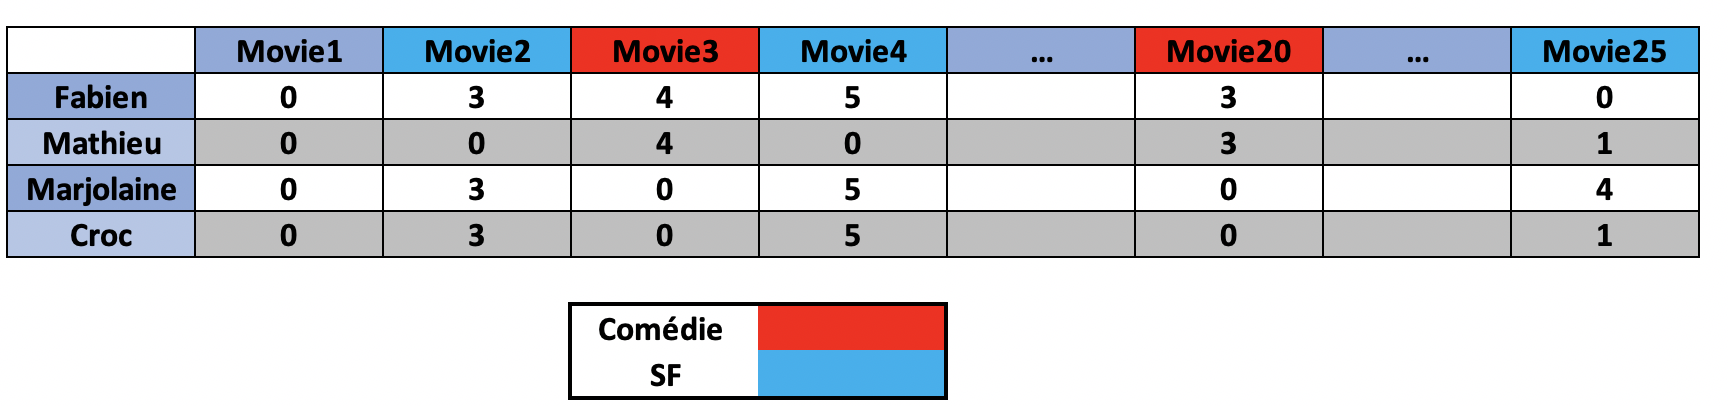
\includegraphics[width=95mm]{./src_img/apport_data}
  \caption{Schéma des données utilisateurs utilisé.}
  \label{fig:a-un}
\end{figure}

\vspace{5mm}

Hormis le profil de « Fabien », nous avons 3 profils utilisateurs. L’utilisateur « Mathieu » est très client des comédies, il a consommé deux films de types Comédie et un film de Science-Fiction le film « movie25 » qu’il n’a malheureusement pas apprécié.  Les profils « Marjolaine » et « Croc » sont friands des films de Science-Fiction, seul leurs notes attribuées au film « movie25 » diffères. 

\vspace{5mm}

Hormis son manque de notation pour « movie25 », le profil  « Fabien » est similaire aux autres profils consommant ainsi des films de Science-fiction et de Comédie. Mon système de recommandation crée en Python aura pour but de prédire la note que Fabien attribuera au film numéro 25 correspondant à "Jurassic World". 


\section{Recherche des plus proches voisins}

Rechercher les plus proches voisins est une méthode très efficace pour créer un groupe d’utilisateur avec des consommations identiques permettant ainsi une recommandation rapide pour un utilisateur donné. Pour rappel, cette méthode a démontré son efficacité lors du Netflix Prize. 

\vspace{5mm}

Concrètement, je prends le  « profil Fabien » et je calcule la distance euclidienne entre les notes attribuées par Fabien et les autres utilisateurs. Mon algorithme des plus proches voisins à une condition supplémentaire, la distance entre Fabien et un autre utilisateur est calculée pour chaque film individuellement et seulement si les deux personnes ont regardé le film sélectionné. La valeur cumulée de la distance euclidienne pour chaque film permet d’obtenir une distance entre Fabien et les autres utilisateurs.  A la fin de cette étape, j’ai une liste de profil organisée de la façon suivante : 

\begin{verbatim}
Distance : données de l’utilisateur Mathieu 
\end{verbatim}

Ensuite, je trie cette liste pour obtenir une liste ordonnée de façon croissante sur la distance. Mais avec ce jeu de données réfléchi, la distance entre Fabien et les autres profils est identique avec une valeur égale à 0, ce qui implique des profils similaires. Au préalable, j’ai défini une limite d’acceptation, dans le cadre de ce mémoire, j’ai choisi de garder les 3 profils les plus proches de l’utilisateur Fabien. 

\vspace{5mm}
 
Ainsi, à la fin de cette étape, les profils :  « Marjolaine, Croc et Mathieu »  sont considérés comme des voisins proches sur lequel une recommandation est possible pour Fabien. 

\begin{figure}[htp]
  \centering
  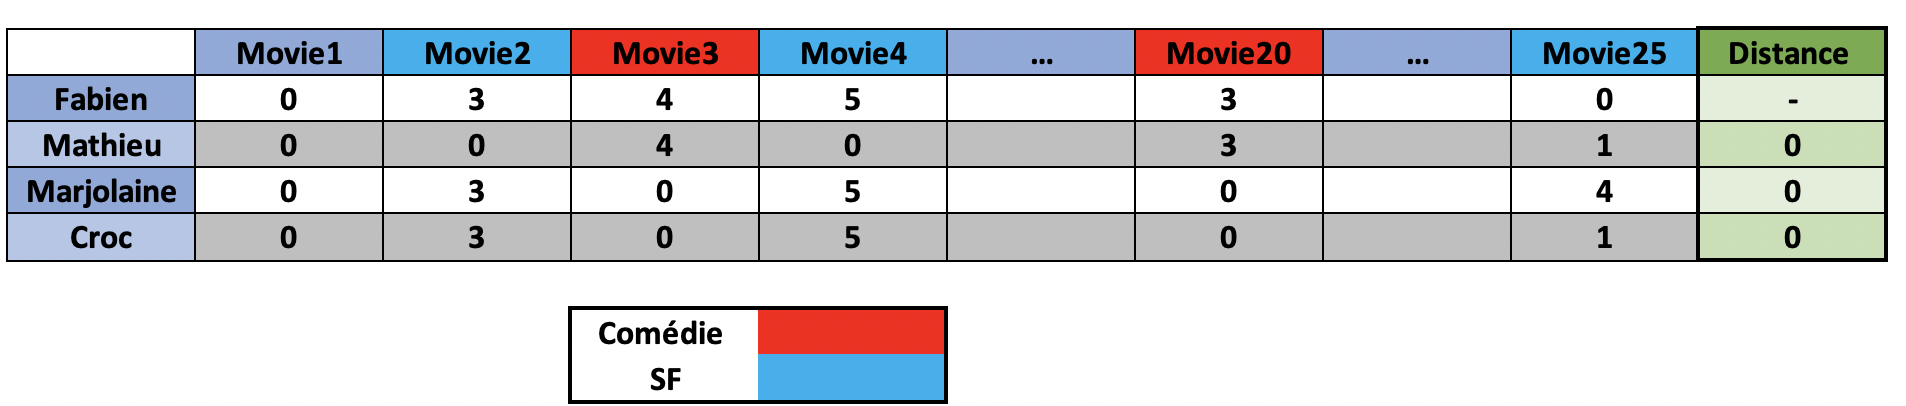
\includegraphics[width=95mm]{./src_img/apport_distance}
  \caption{Recherche des plus proches voisins.}
  \label{fig:a-deux}
\end{figure}

\vspace{5mm}


\section{Trier les voisins selon le film}

En partant des données pour Fabien et sa liste des plus proches voisins, mon système de recommandation va essayer de recommander un ou plusieurs films pour Fabien. Techniquement, pour chaque film non regardé par Fabien, je vais rechercher si parmis ses voisins les plus proches au moins un voisin a regardé ce film. Dans ce cas précis, seul le film "Jurassic World" (« Movie25 ») est éligible.

\vspace{5mm}

Premièrement, je vais enlever de la liste des voisins les plus proches ceux qui n’ont pas regardé ce film. Dans notre cas très précis, aucun voisin n’est évincé. Deuxièmement, je vais appliquer une variante de l’algorithme des plus proches voisins mais basé sur le type du film. Concrètement, "Jurassic World" est un film de Science-Fiction et je vais calculer la note moyenne attribué par Fabien sur les films de type Science-Fiction. Cette moyenne est aussi calculée pour chaque voisin proche restant. 

\vspace{5mm}

Finalement, il faut classer les voisins restant selon leur moyenne attribuée aux films de Science-fiction et non pas par ordre croissant mais selon si leur moyenne est proche ou non de celle de Fabien. Donnant le résultat suivant : 

\vspace{5mm}


\begin{figure}[htp]
  \centering
  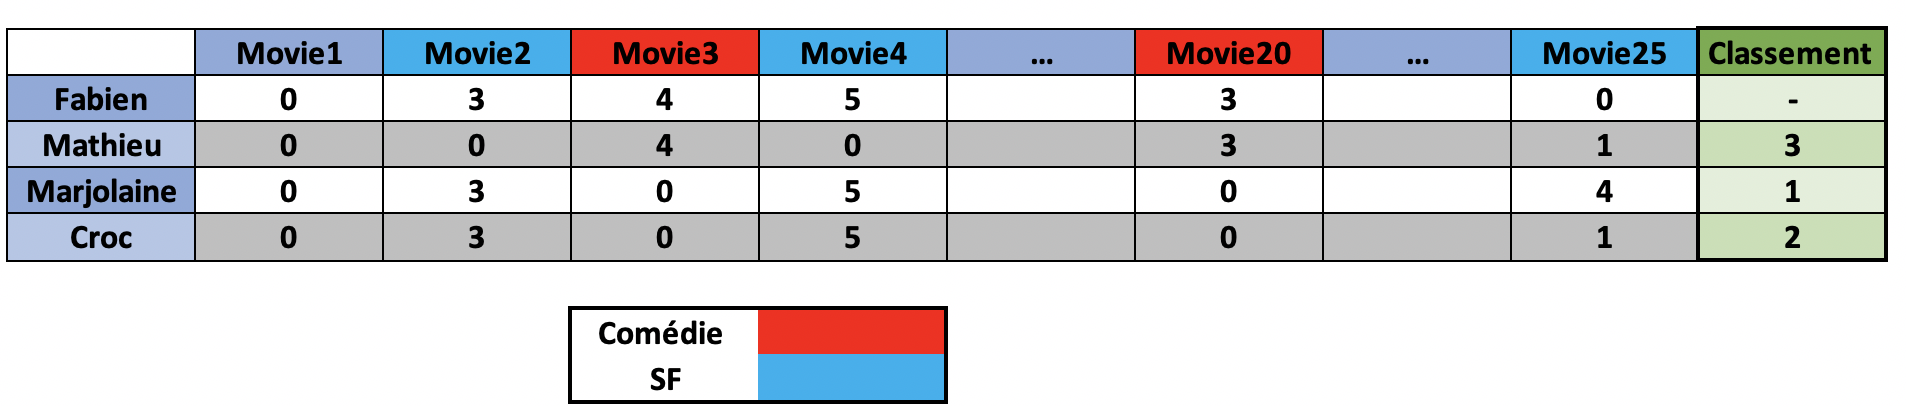
\includegraphics[width=95mm]{./src_img/apport_classement}
  \caption{Classement des voisins.}
  \label{fig:a-trois}
\end{figure}

\vspace{5mm}

\section{Prédiction}

Dans cette section, il faut prendre en compte plusieurs paramètres. Notamment si le genre du film sur lequel le système travaille à déjà au moins une évaluation par Fabien. On distingue deux cas : 

\vspace{5mm}

Le premier cas, si Fabien a déjà évalué au moins un film de Science-fiction, alors il faut calculer la différence entre la moyenne attribuée par Fabien au genre Science-fiction et la moyenne du voisin sélectionné pour ce même genre. Dans le cadre de mon développement, j’ai transformé la différence entre ces deux moyennes en un multiplicateur appelé « delta ». Le delta vaut exactement 1 si les deux utilisateurs ont une moyenne identique, le delta est négatif si Fabien note plus faiblement que le voisin sélectionné et inversement le delta est positif si Fabien note plus généreusement. Finalement, pour prédire la note du film, il faut multiplier la note donnée par le voisin par le delta. 

\vspace{5mm}

Le second cas, si Fabien n’a jamais attribué une note aux films de Science-fiction. Une moyenne donnée par Fabien pour le genre Science-fiction est impossible. J’ai choisi d’appliquer la même méthodologie que pour le premier cas mais sur les notes données de façon globale. Ainsi, je vais calculer la moyenne de toutes les notes données par Fabien et le voisin sélectionné. A partir des deux moyennes comme dans le premier cas, je vais créer un delta entre les deux moyennes. Finalement, pour prédire la note du film, il faut multiplier la note donnée par le voisin par le delta. 

\vspace{5mm}

Dans notre cas, Fabien a déjà attribué des notes à des films de Science-fiction avec une moyenne de 4 pour ce genre de film. Le profil voisin le plus proche est Marjolaine avec une moyenne de 4 attribuée sur les films de Science-fiction. Ici, le delta entre les deux moyennes à pour valeur 1 et Marjolaine a attribué la note de 4 au film "Jurassic World". Par conséquent, le système prédit que Fabien va attribuer une note de 4 pour le film "Jurassic World". 

\begin{verbatim}
Predict for Fabien
- - - - - - - - - - - - - - - - - - -
[0, 3, 4, 5, 0, 0, 0, 0, 0, 0, 0, 0, 0, 0, 0, 0, 0, 0, 0, 3, 0, 0, 0, 0, 4]
new rating : 4  
['Movie25', '2015', 'Jurassic World', 'Science-Fiction']
- - - - - - - - - - - - - - - - - - -
\end{verbatim}